\documentclass[12pt]{article}

\usepackage[UTF8]{ctex}
\usepackage{appendix}
\usepackage{enumerate}
\usepackage{amsmath}
\usepackage{graphicx}
\usepackage{cite}
\usepackage{array}
\usepackage{caption}
\usepackage{bigstrut}
\usepackage{geometry}
\geometry{left =2.5 cm,right=2.5cm,top=2.5cm,bottom=2.5cm}
\usepackage{multirow}
\usepackage{lastpage}
\usepackage{longtable}
\usepackage{listings}
  \usepackage{textcomp} % 必须加上,否则报错
  \usepackage[framed,numbered,autolinebreaks,useliterate]{mcode}    % 添加matlab代码宏
  \usepackage{xcolor}
  \lstset{
  language=Matlab,  %代码语言使用的是matlab
  rulesepcolor=\color{red!20!green!20!blue!20},%代码块边框为淡青色
  keywordstyle=\color{blue!90}\bfseries, %代码关键字的颜色为蓝色,粗体
    numbers=left, % 显示行号
    numberstyle=\tiny,    % 行号字体
   commentstyle=\color[RGB]{0,130,0},    % 设置代码注释的颜色
  showstringspaces=false,%不显示代码字符串中间的空格标记
  stringstyle=\ttfamily, % 代码字符串的特殊格式
  breaklines=true, %对过长的代码自动换行
  extendedchars=false,  %解决代码跨页时,章节标题,页眉等汉字不显示的问题
  escapeinside=``,      % 代码中出现中文必须加上,否则报错
  texcl=true,}
  \lstset{breaklines}
\usepackage[section]{placeins}
\usepackage[colorlinks,linkcolor=blue]{hyperref}
\usepackage{titlesec}
\usepackage{titletoc}
\titleformat{\section}{\centering\heiti\zihao{3}}{实验\thesection}{0.3em}{}
\titleformat{\subsection}{\heiti \fontsize{12pt}{0}}{\thesubsection}{0.3em}{}
\renewcommand\figurename{\heiti\zihao{5} 图}
\renewcommand\tablename{\heiti\zihao{5} 表}
\renewcommand {\thetable} {\thesection{}.\arabic{table}}
\renewcommand {\thefigure} {\thesection{}.\arabic{figure}}

\date{}
\geometry{a4paper,scale=0.8}

\begin{document}%文档从这里开始。
\captionsetup{labelformat=default,labelsep=space}
\numberwithin{footnote}{section}
\renewcommand{\contentsname}{\centering 目录}
%\renewcommand{\tablename}{表}
%\renewcommand{\figurename}{图}
\renewcommand\refname{参考文献}
\renewcommand\appendix{\setcounter{secnumdepth}{0}}
\renewcommand\abstractname{摘要}
\begin{figure}[h]
  \centering
  
\includegraphics[width=.6\textwidth]{logo}
\end{figure}
\thispagestyle{empty}
\begin{center}
\begin{songti}
\zihao{0}\textbf{数字图像处理}\\
\zihao{0}\textbf{实验报告}\\\ \\\
\zihao{3}
\\ \
\renewcommand\arraystretch{1.5}
\begin{tabular}{p{1.5cm}<{\centering} p{0.2cm}<{\centering} p{3.5cm}<{\centering} p{1.5cm}<{\centering} p{0.2cm}<{\centering} p{3.5cm}<{\centering}}
课程&\textbf{:}&\multicolumn{4}{c}{数字图像处理}\\\cline{3-6}
教师&\textbf{:}&\multicolumn{4}{c}{张玉珍}\\\cline{3-6}
组号&\textbf{:}&\multicolumn{4}{c}{第9组}\\\cline{3-6}
组员&\textbf{:}&许婷&学号&\textbf{:}&9161040G0508\\\cline{3-3}\cline{6-6}
组员&\textbf{:}&孙宏寰&学号&\textbf{:}&9161040G0707\\\cline{3-3}\cline{6-6}
组员&\textbf{:}&董建博&学号&\textbf{:}&9161040G0718\\\cline{3-3}\cline{6-6}
组员&\textbf{:}&许晓明&学号&\textbf{:}&9161040G0734\\\cline{3-3}\cline{6-6}
组员&\textbf{:}&周茂源 &学号&\textbf{:}&9161040G0809\\\cline{3-3}\cline{6-6}
\end{tabular}

\begin{table}[b]
  \centering
\number\year\ 年\ \number\month月
\end{table}

\end{songti}
\end{center}
\begin{center}
\newpage
%\raggedright
\zihao{4}
\newpage
\setcounter{page}{1}
\pagenumbering{Roman}
\tableofcontents
\newpage
\setcounter{page}{1}

\end{center}

\setcounter{page}{1}
\pagenumbering{arabic}
\section{数字图像处理线性增强}
\subsection{实验目的}
编写线性增强的C或C++或MATLAB语言程序及相应显示程序。
\subsection{实验内容}
利用MATLAB实现图像线性增强。
\subsection{实验过程}
\begin{enumerate}
  \item 首先通过imread读取一张彩色图片。
\item 将彩色图像进行线性变换
\item 通过matlab的内置函数将彩色图转换成灰度图。
\item 判断图像X的大小,再通过for循环遍历图片中的每一个像素,通过函数进行线性变换
\end{enumerate}
\subsection{实验代码}
\begin{lstlisting}
clc;
R=imread('蛋糕.jpg');
H=2+1.35*(R-2);%线性变换
X=rgb2gray(R);%将真彩色RGB图像转换成灰度图像
[a,b]=size(X);
for i=1:a-1
for j=1:b-1
I(i,j)=2+1.35*(X(i,j)-2);
end
End
subplot(231);imshow(R);title('原始图像');
subplot(232);imshow(uint8(H));title('增强图像');
subplot(233);imshow(X);title('灰度图像');
subplot(234);imhist(X,256);title('原图直方图');
subplot(235);imhist(I,256);title('增强直方图');
hold on;
x=[0:5];
y=2+1.35*(x-2);
subplot(236);plot(x,y);title('函数图像');
\end{lstlisting}
\subsection{实验结果}
实验结果见图\ref{shiyan1}。
\begin{figure}[h]
  \centering
  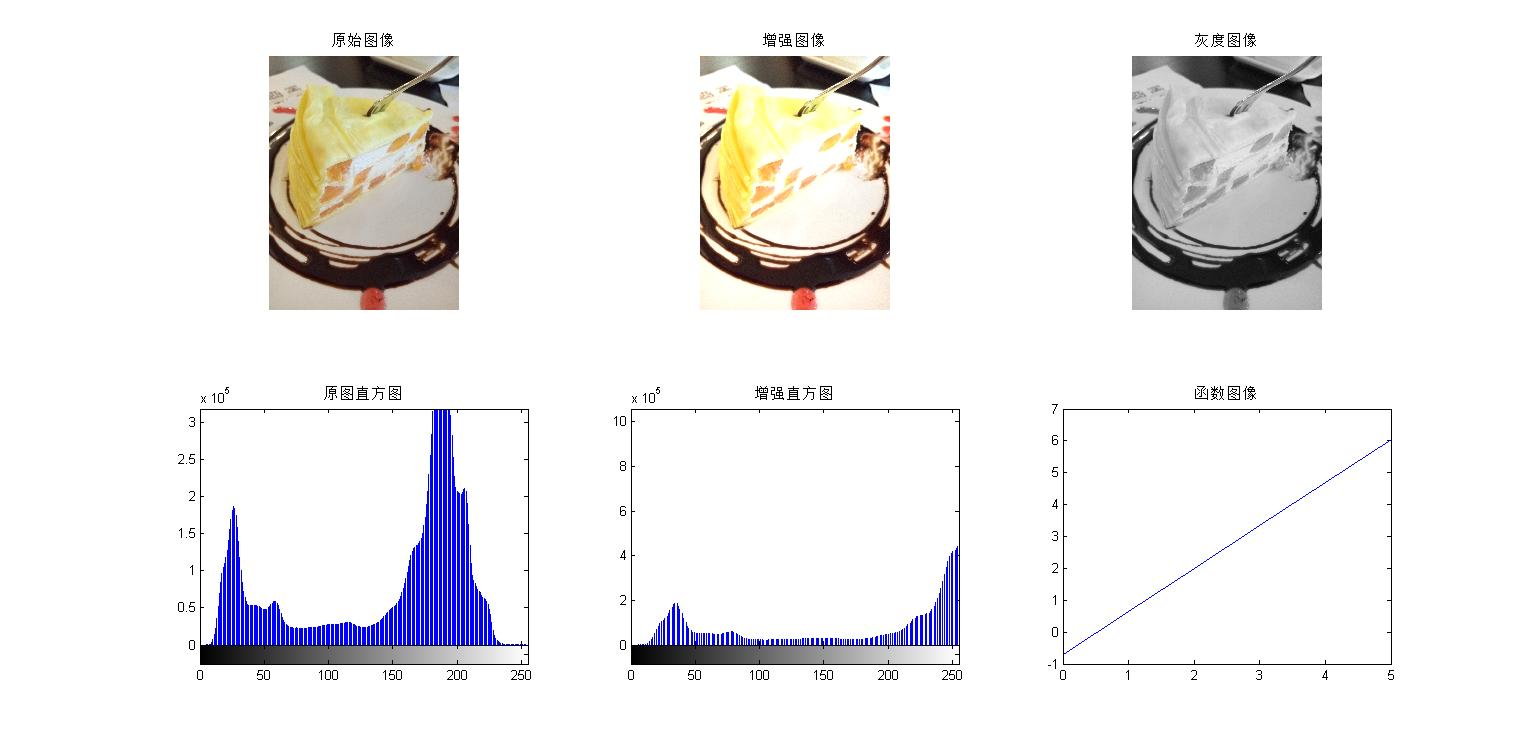
\includegraphics[width=\textwidth]{picture/xianxingzengq.jpg}
  \caption{}\label{shiyan1}
\end{figure}
\subsection{实验分析}
该实验属于图像增强的线性变换部分。通过变换使图像的动态范围增大,图像对比度扩展,图像变清晰,特征明显。通过直方图看出,图像在变换前灰度过于集中在一个部分,变换后对图像的每一像素进行了拉伸,灰度值分布均匀,有效的改善了图像视觉效果。
\newpage
\section{数字图像处理中值滤波}
\setcounter{equation}{0}
\setcounter{table}{0}
\setcounter{figure}{0}
\subsection{实验目的}
掌握中值滤波的基本原理, 熟悉中值滤波的方法。
\subsection{实验内容}
编写中值滤波及图像平滑化的matlab语言程序以及相应的显示程序和原图比较,分析四点平滑滤波图像平滑化后的效果。
\subsection{实验原理}
中值滤波是基于排序统计理论的一种能有效抑制噪声的非线性信号处理技术,中值滤波的基本原理是把数字图像或数字序列中一点的值用该点的一个邻域中各点值的中值代替,让周围的像素值接近的真实值,从而消除孤立的噪声点。方法是用某种结构的二维滑动模板,将板内像素按照像素值的大小进行排序,生成单调上升(或下降)的为二维数据序列。二维中值滤波输出为$$g(x,y)={\rm med} {f(x-k,y-l),(k,l\in W)}$$  其中,$f(x,y),g(x,y)$分别为原始图像和处理后图像。W为二维模板,通常为$3\times 3,5\times 5$区域,也可以是不同的的形状,如线状,圆形,十字形,圆环形等。\par
具体流程如下:
\begin{enumerate}
  \item 通过从图像中的某个采样窗口取出奇数个数据进行排序
 \item 用排序后的中值取代要处理的数据即可
\end{enumerate}
\subsection{实验步骤}
\begin{enumerate}
  \item 新建 matlab 工程;
\item 分析程序流程;
\item 编写程序;
\item 运行调试;
\item 显示结果;
\item 分析结果。
\end{enumerate}

\subsection{实验代码及解释}
中值滤波程序
\begin{lstlisting}
A=imread('beijing.jpg'); %读取北京图片
J=rgb2gray(A);%将RGB彩色图像转化为灰度图,减少运算量,提高运算速度
subplot(1,2,1);
P1=imnoise(J,'salt&pepper',0.03)%对图像生成椒盐噪声
imshow(P1)
title('原图像')
[m,n]=size(J) ;                 %取得原图矩阵尺寸
B=zeros(9);%生成9*9的全零方阵
for i=2:m1                     %从第二个开始到倒数第二个结束
for j=2:n-1
b=1;
for p=(i-1):(i+1)%取小框3行
for q=(j-1):(j+1)%取小框3列
B(b)=J(p,q);%将选中3*3的值赋给B
b=b+1;
end
end
for d=1:8          %开始冒泡程序
if(B(d)>B(d+1))%由小到大排序,大则交换,否则不交换
t=B(d);
B(d)=B(d+1);
B(d+1)=t;
end
end
J(i,j)=B(5,1);  %将排序后的像素值赋给J
end
end
subplot(1,2,2);
imshow(J)
title('中值滤波后 ')
\end{lstlisting}
为对比中值滤波对椒盐噪声和高斯噪声的作用效果,改进程序如下
\begin{lstlisting}
clc
A=imread('beijing.jpg');
J=rgb2gray(A);
E=J;
subplot(3,2,5);
imshow(E);
title('原图像')
P1=imnoise(J,'gaussian',0.2);%对图像生成高斯噪声
subplot(3,2,2);
imshow(P1)
title('高斯原图像 ')
[m,n]=size(J) ;
B=zeros(9);
for i=2:m-1
for j=2:n-1
b=1;
for p=(i-1):(i+1)
for q=(j-1):(j+1)
B(b)=J(p,q);
b=b+1;
end
end
for d=1:8
if(B(d)>B(d+1))
t=B(d);
B(d)=B(d+1);
B(d+1)=t;
end
end
J(i,j)=B(5,1);
end
end
subplot(3,2,4);
imshow(J)
title('高斯噪声中值滤波后 ')
C=rgb2gray(A);
subplot(3,2,1);
P2=imnoise(C,'salt&pepper',0.2);%对图像生成椒盐噪声
imshow(P2)
title('椒盐原图像')
[x,y]=size(C) ;
D=zeros(9);
for i=2:x-1
for j=2:y-1
b=1;
for p=(i-1):(i+1)
for q=(j-1):(j+1)
D(b)=C(p,q);
b=b+1;
end
end
for d=1:8
if(D(d)>D(d+1))
t=D(d);
D(d)=D(d+1);
D(d+1)=t;
end
end
C(i,j)=D(5,1);
end
end
subplot(3,2,3);
imshow(C)
title('椒盐噪声中值滤波后 ')
\end{lstlisting}

\subsection{实验结果}
实验结果见图\ref{jiaoyan1}$\sim$图\ref{jiaoyan2}
。
\begin{figure}[htbp]
  \centering
  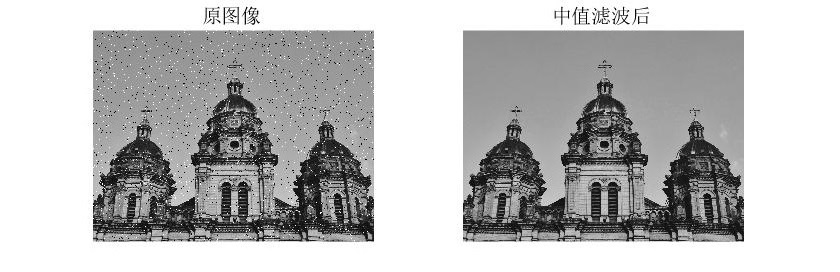
\includegraphics[width=\textwidth]{picture/jiaoyanzhongzhilvbo}
  \caption{}\label{jiaoyan1}
\end{figure}
\begin{figure}[htbp]
  \centering
  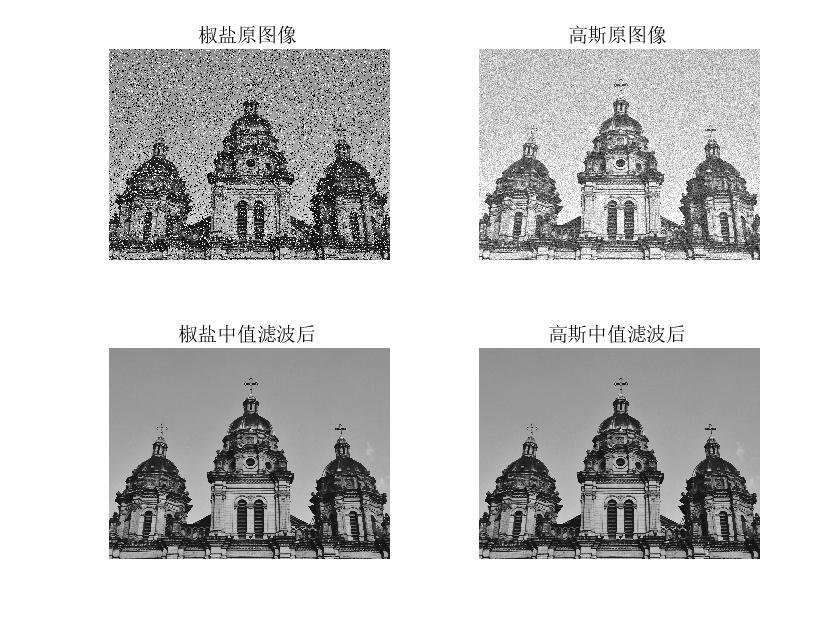
\includegraphics[width=\textwidth]{picture/gaosijiaoyanzhongzhilvbo}
  \caption{}\label{jiaoyan2}
\end{figure}
\subsection{实验分析}
因为中值滤波的原理是取合理的邻近像素值来代替噪声点,所以只适用于椒盐噪声的去除。\par
但适当选取模板的大小(或结构形状)也很重要,将上述程序的$3\times 3$模板改变扩大为$7\times 7$或更大,图像的清晰度就遭到了破坏。\par
理论上来说,中值滤波对于椒盐噪声的效果应该好于高斯噪声。
\newpage
\section{数字图像直方图均衡化处理}
\setcounter{equation}{0}
\setcounter{table}{0}
\setcounter{figure}{0}
\subsection{实验目的}
通过了解直方图的绘制、均衡化的基本原理与实现方法,熟悉在计算机上进行直方图均衡化、线性变换的方法,来掌握简单的直方图均衡化和线性变换程序设计编写。
\subsection{实验内容}
编写直方图的显示、均衡化的matlab语言程序,同时显示变换后的直方图。
\subsection{实验原理}
直方图均衡化处理的中心思想是把原始图像的灰度直方图从比较集中的某个灰度区间变成在全部灰度范围内的均匀分布。通过对图像进行非线性拉伸,重新分配图像像素值,使一定灰度范围内的像素数量大致相同,把给定图像的直方图分布改变成“均匀”分布直方图分布。\par
利用累积分布函数,完成原图像直方图均匀分布的效果。
\subsection{实验步骤}
\begin{enumerate}
  \item 新建工程;
\item 分析程序流程;
\item 编写程序;
\item 运行调试;
\item 显示结果;
\item 分析结果。
\end{enumerate}
\subsection{实验代码}
\begin{lstlisting}
close all;clear all;clc;
A= imread('E:\baogao\数字图像处理\picture\IMG_20190314_194136.jpg');
original=rgb2gray(A);%转灰度
[h w] = size(original); %获取待处理图片尺寸
p=zeros(6,256);
f=zeros(1,256);%统计每个像素值出现次数
for i=1:1:h
for j=1:1:w
for k=0:1:255
if original(i,j)==k
p(1,k+1)=p(1,k+1)+1;
end
end
end
end%计算概率直方图
for i=1:1:256
p(2,i)=p(1,i)/(h*w);
end     %求累计概率,得到累计直方图
p(3,1)=p(2,1);
for i = 2 : 256
p(3, i) = p(3, i - 1) + p(2, i);
end%用p3数组实现灰度值[0, 255]的映射
for i = 1:1:256
f(i) = round(p(3, i) * 255);
end %直方图均衡化
equalize=uint8(zeros(h,w));
for i=1:1:h
for j=1:1:w
for k=0:1:255
if original(i,j)==k
equalize(i,j)=f(k+1) ;
end
end
end
end%统计每个像素值出现次数
for i=1:1:h
for j=1:1:w
for k=0:1:255
if equalize(i,j)==k
p(4,k+1)=p(4,k+1)+1;
end
end
end
end%计算新的概率直方图
for i=1:1:256
p(5,i)=p(4,i)/(h*w);
end%求累计概率,得到新的累计直方图
p(6,1)=p(5,1);
for i = 2 : 256
p(6, i) = p(6, i - 1) + p(5, i);
end
subplot(231)
imshow(original)
title('原图');
subplot(232)
bar(p(2,:))
xlim([0,256]);
set(gca,'XGrid','on');
set(gca,'YGrid','on');
title('原概率直方图');
subplot(233)
bar(p(3,:))
xlim([0,256]);
set(gca,'XGrid','on');
set(gca,'YGrid','on');
title('原累计直方图');
subplot(234)
imshow(equalize)
title('直方图均衡化');
subplot(235)
bar(p(5,:))
xlim([0,256]);
set(gca,'XGrid','on');
set(gca,'YGrid','on');
title('新的概率直方图');
subplot(236)
bar(p(6,:))
xlim([0,256]);
set(gca,'XGrid','on');
set(gca,'YGrid','on');
title('新的累计直方图');
\end{lstlisting}
\subsection{实验结果}
实验结果见图\ref{01}$\sim$
图\ref{04}
。
\begin{figure}[htbp]
  \centering
  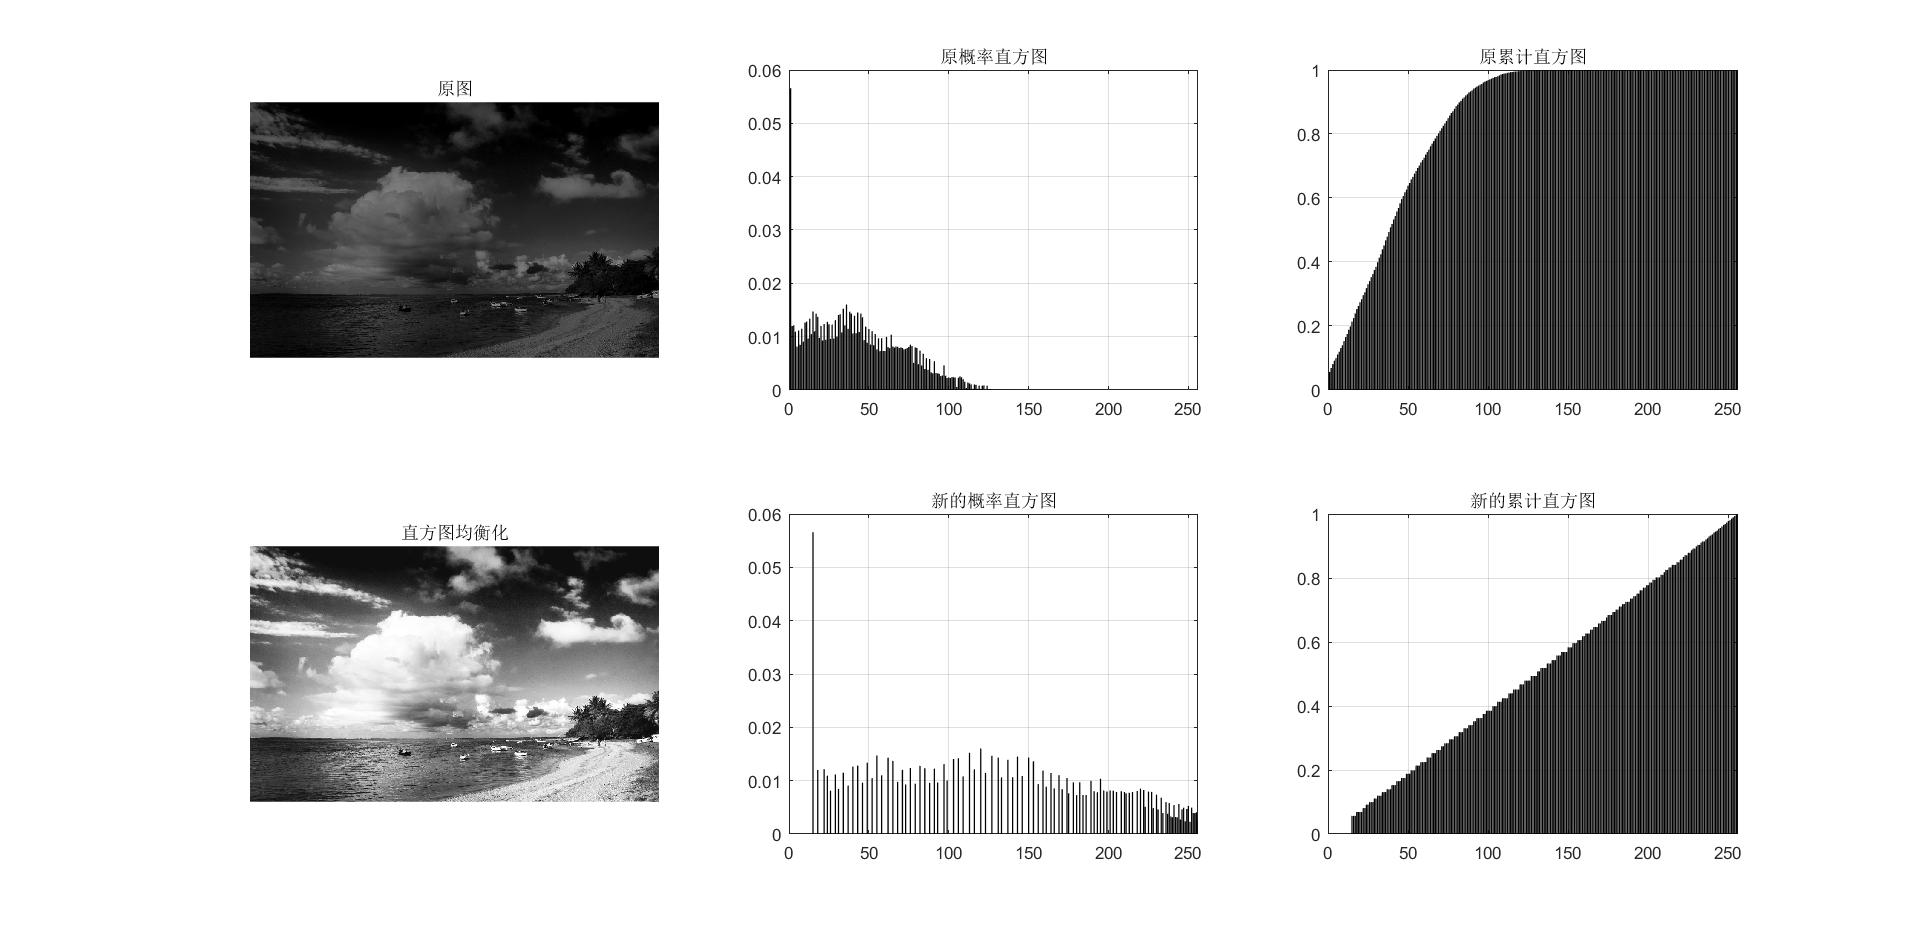
\includegraphics[width=\textwidth]{picture/01}
  \caption{}\label{01}
\end{figure}
\begin{figure}[htbp]
  \centering
  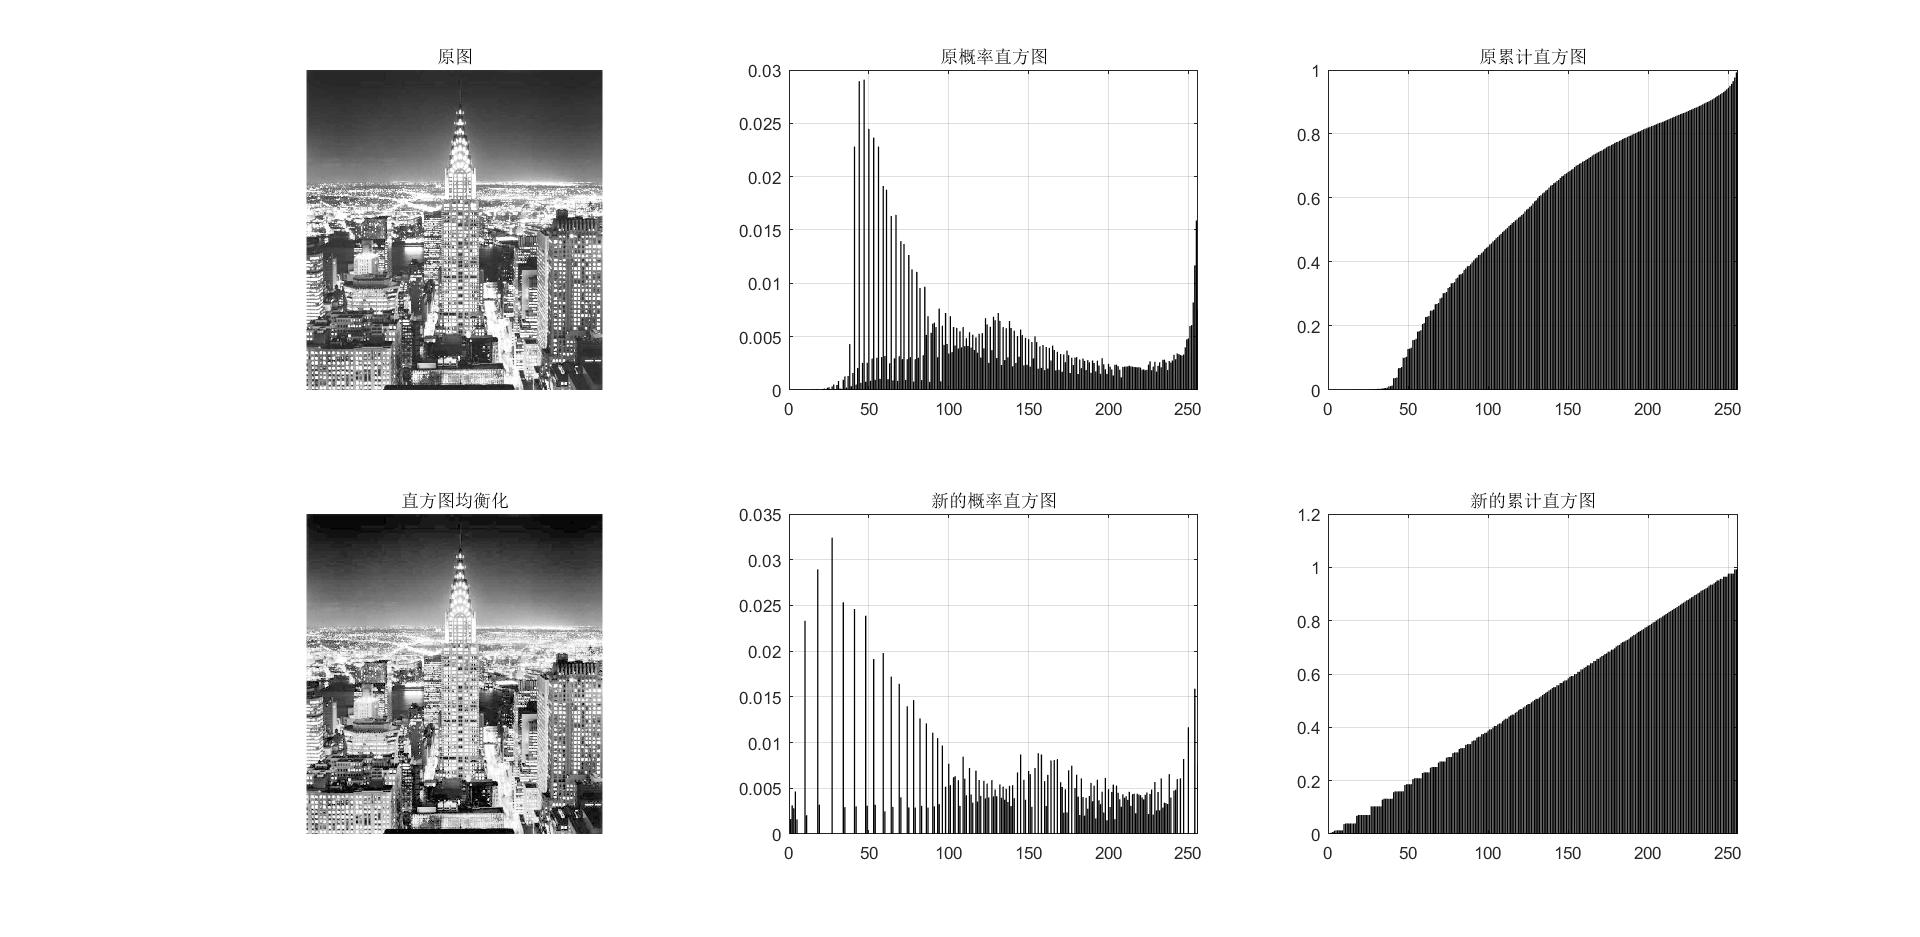
\includegraphics[width=\textwidth]{picture/02}
  \caption{}\label{02}
\end{figure}
\begin{figure}[htbp]
  \centering
  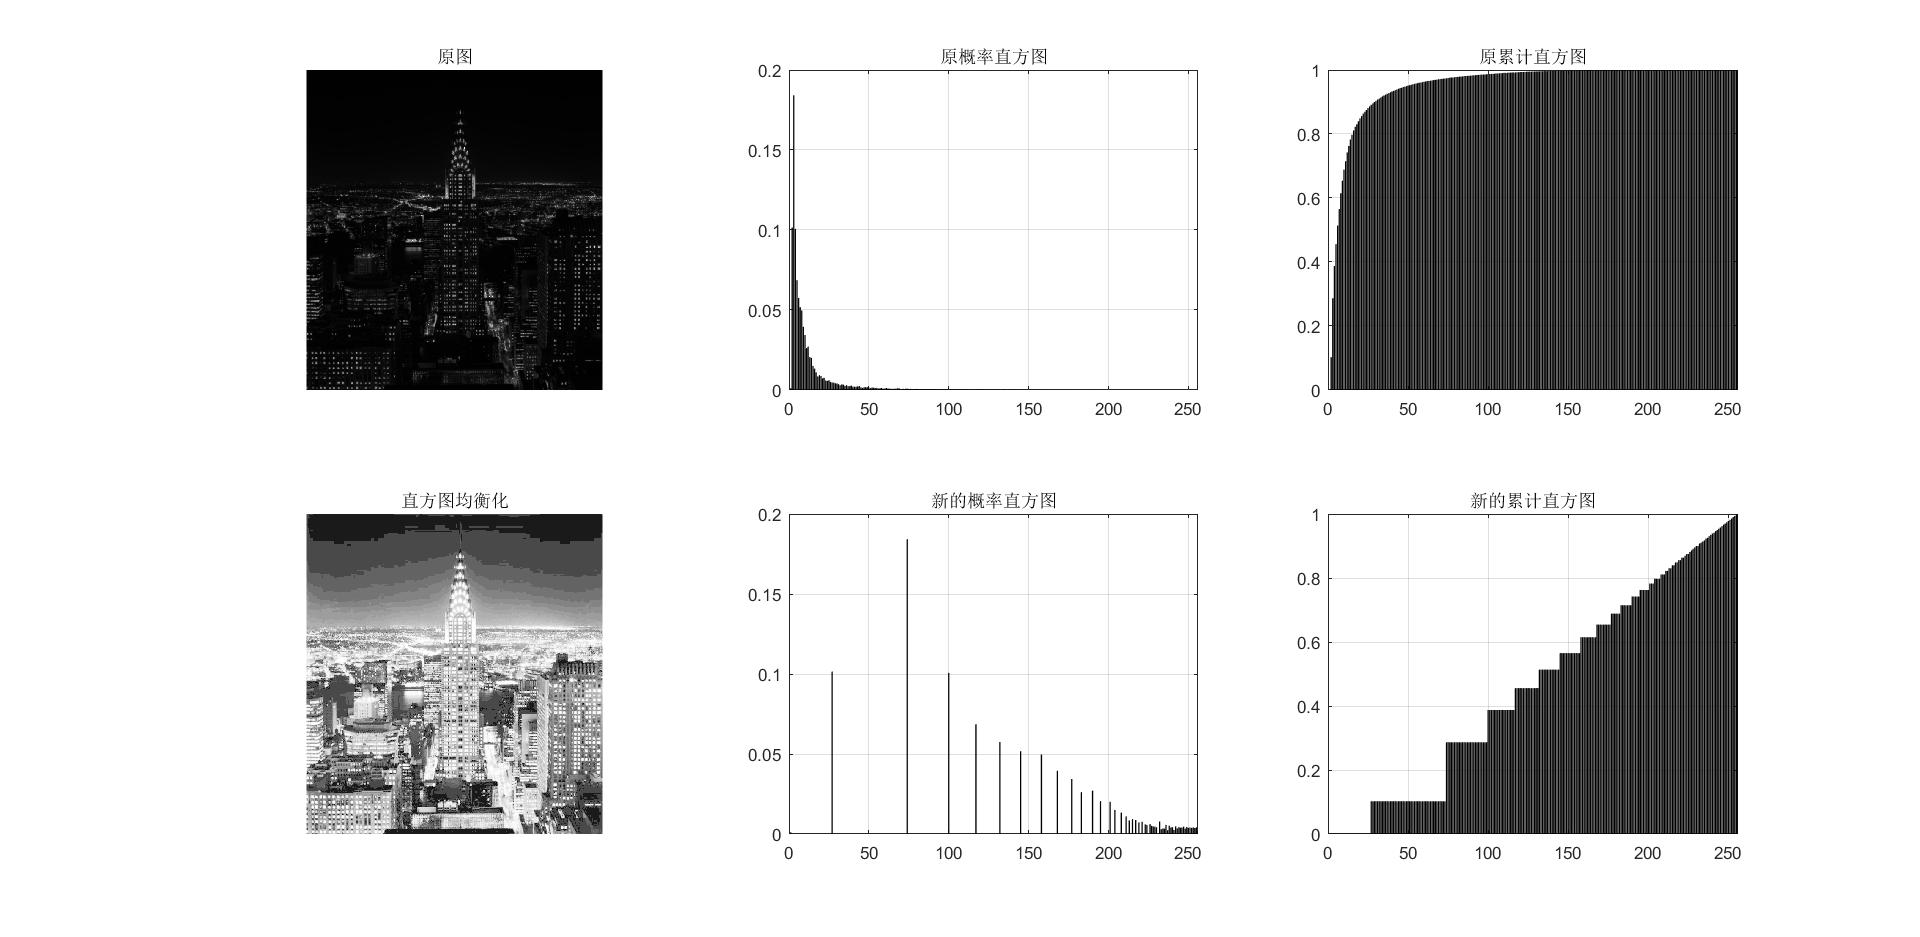
\includegraphics[width=\textwidth]{picture/03}
  \caption{}\label{03}
\end{figure}
\begin{figure}[htbp]
  \centering
  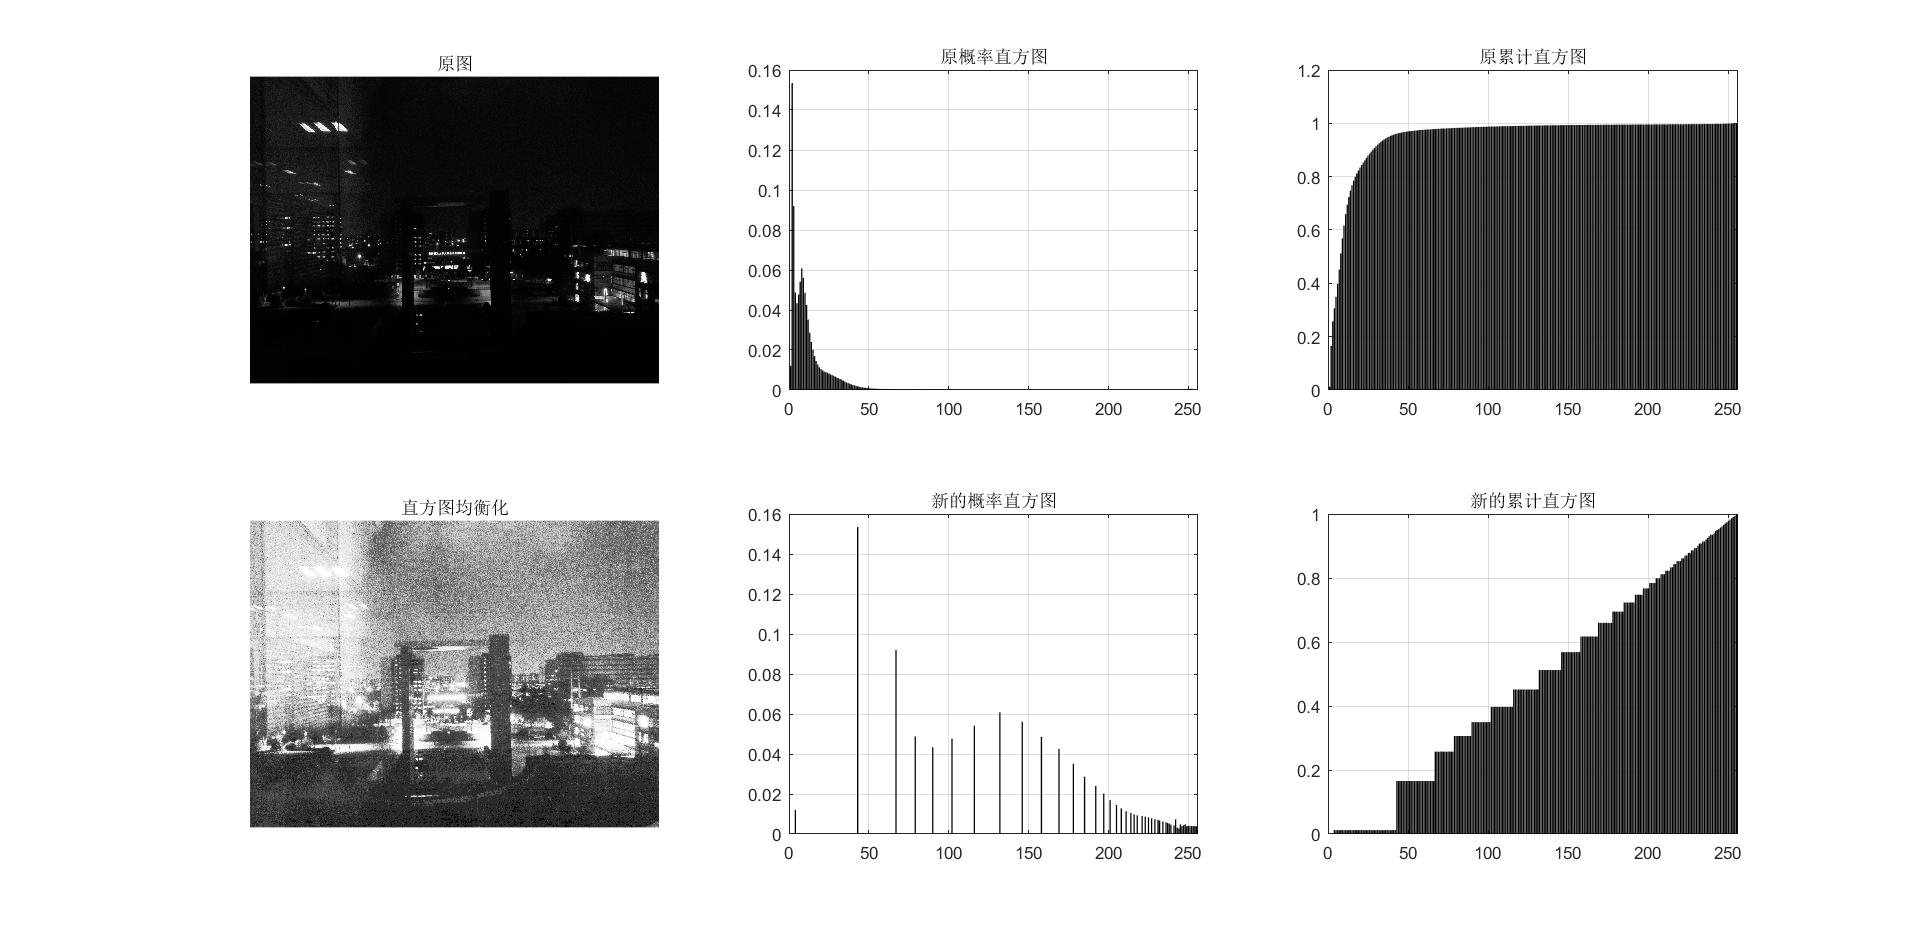
\includegraphics[width=\textwidth]{picture/04}
  \caption{}\label{04}
\end{figure}
\subsection{实验分析}
如图\ref{01}
所示,直方图均衡化对于像素灰度集中在低值区(图片偏灰暗)的图片改善效果较强,但对于如图\ref{02}
的灰度值集中在高值区(图像过曝)的图片,则改善效果不佳。而对于如图\ref{03},\ref{04}
的灰度值过度集中在某一区域的图片,由于直方图均衡化变换后图像的灰度级减少,某些细节消失。尤其是如图\ref{03}
,直方图有高峰,经处理后对比度不自然的过分增强,产生马赫带效应。
\newpage
\section{数字图像处理空间平滑}
\setcounter{equation}{0}
\setcounter{table}{0}
\setcounter{figure}{0}
\subsection{实验目的}
掌握图像平滑基本原理,掌握4点平滑,8点平滑,中值滤波平滑基本原理,掌握计算机软件处理图像的方法。
\subsection{实验内容}
编写4点平滑,8点平滑,中值滤波的C或C++或matlab语言程序以及相应的显示程序。
\subsection{实验步骤}
\begin{enumerate}
  \item 原理过程分析;
\item 程序流程分析;
\item 编写程序;
\item 运行调试;
\item 结果展示;
\end{enumerate}
\subsection{实验原理}
用像素值邻域(4联通或8联通)的平均值代替该店像素值,实现平滑效果,能有效的去除噪声。\par
   数字图像处理中简化为下列公式:
$$B(i,j)=A(i,j-1)/5+A(i,j)/5+A(i,j+1)/5+A(i-1,j)/5+A(i+1,j)/5$$

\[\begin{split}
B(i,j)=A(i,j-1)/9+A(i,j)/9+A(i,j+1)/9+A(i-1,j)/9+A(i+1,j)/9+\\
A(i-1,j-1)/9+A(i+1,j-1)/9+A(i-1,j+1)/9+A(i+1,j+1)/9
\end{split}
\]

\subsection{实验程序}
4点平滑实验代码
\begin{lstlisting}
A=imread('C:\Users\loveless\Documents\MATLAB\reflection.jpg');%     读入图像
I=imnoise(A,'salt & pepper',0.025);%       加入椒盐噪声
subplot(1,2,1);imshow(I);title('原图像');%       显示原图像
[a,b]=size(I); %     读取图像尺寸大小
J=double(I);

for i=2:a-1%   处理图像矩阵
for j=2:b-1
J(i,j)=(J(i-1,j)+J(i,j+1)+J(i+1,j)+J(i,j-1))/4; %4点均值
end
end
J=uint8(J);
subplot(1,2,2);imshow(J);title('4点均值平滑后的图像');%显示处理后的图像
\end{lstlisting}
8点平滑实验代码
\begin{lstlisting}
A=imread('C:\Users\loveless\Documents\MATLAB\reflection.jpg');%读入图像
I=imnoise(A,'salt & pepper',0.025);%加入椒盐噪声
[a,b]=size(I); %读取图像尺寸大小
J=double(I);
for i=2:a-1
for j=2:b-1
J(i,j)=(J(i-1,j-1)+J(i-1,j)+J(i-1,j+1)+J(i,j-1)+...
J(i,j+1)+J(i+1,j-1)+J(i+1,j)+J(i+1,j+1))/8;%8点均值
end
end
J=uint8(J);
subplot(1,2,1);imshow(I);title('原图像');%显示加噪声后的图像
subplot(1,2,2);imshow(J);title('8点均值平滑后的图像');%显示处理后的图像
\end{lstlisting}
\subsection{实验结果}
4点平滑显示结果见图\ref{4p}
,8点平滑显示结果见图\ref{8p}
。
\begin{figure}[htbp]
  \centering
  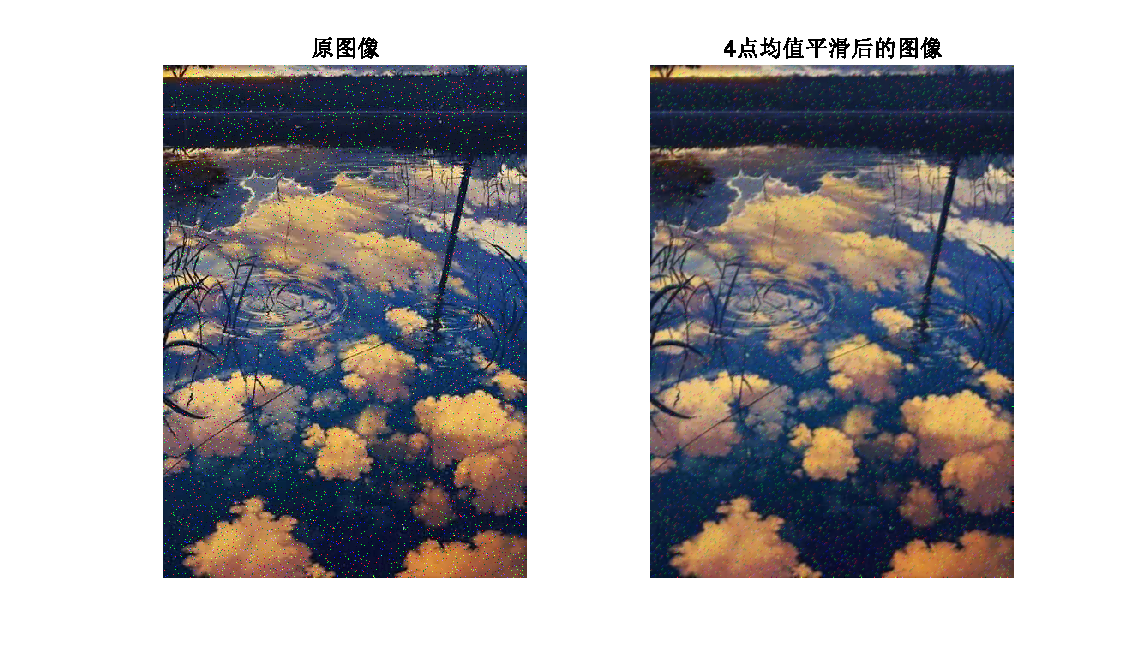
\includegraphics[width=\textwidth]{picture/4points}
  \caption{}\label{4p}
\end{figure}
\begin{figure}[htbp]
  \centering
  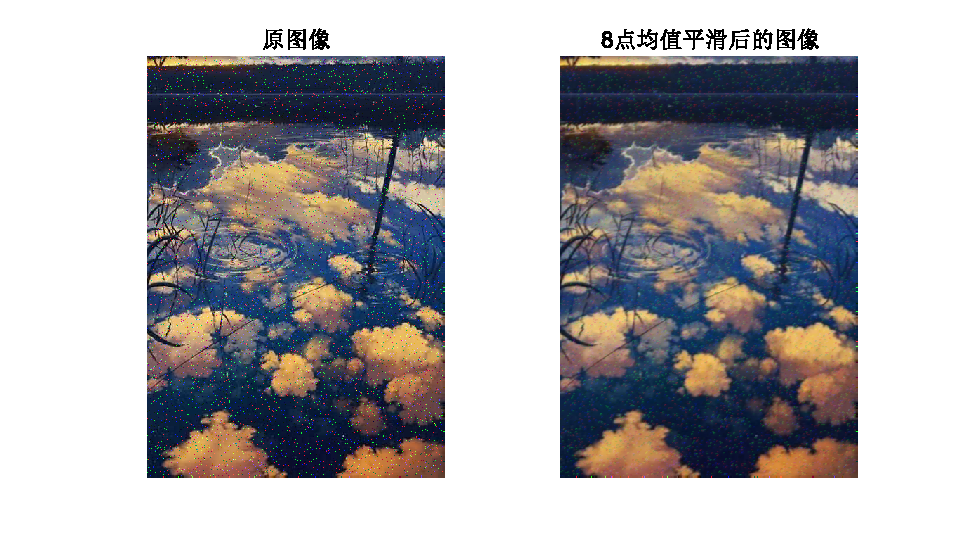
\includegraphics[width=\textwidth]{picture/8points}
  \caption{}\label{8p}
\end{figure}
\appendix
\titleformat{\section}{\heiti\zihao{4}}{}{0.3em}{}
\section{分工情况}
\begin{table}[htbp]
  \centering
  \caption{第9组实验分工表}
    \begin{tabular}{cc}
    \hline
    组员 & 分工 \\
    \hline
    许婷 & 数字图像处理线性增强 \\
    孙宏寰 & 数字图像处理空间平滑 \\
    董建博 & 报告撰写 \\
    许晓明 & 数字图像直方图均衡化处理 \\
    周茂源  & 数字图像处理中值滤波 \\
    \hline
    \end{tabular}%
  \label{tab:addlabel}%
\end{table}%
\end{document}
